\documentclass[]{article}

\usepackage{graphicx}

%opening
\title{3D-printable micropipette}
\author{}

\begin{document}

\maketitle

\begin{figure}
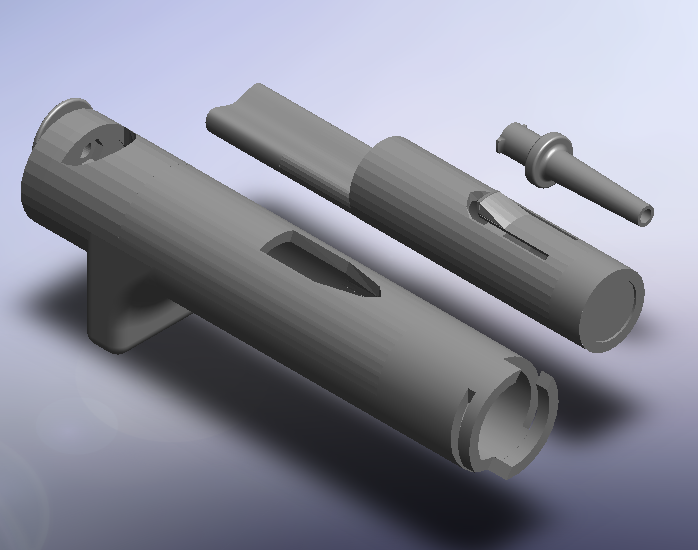
\includegraphics[scale=0.4]{fig1.PNG} % take image out for final manuscript
\caption{
{\bf CAD rendering of printable parts.}  Three parts are printed: the body, plunger shaft, and luer-lock adapter for pipette tips.
}
\label{figure1}
\end{figure}

\begin{figure}
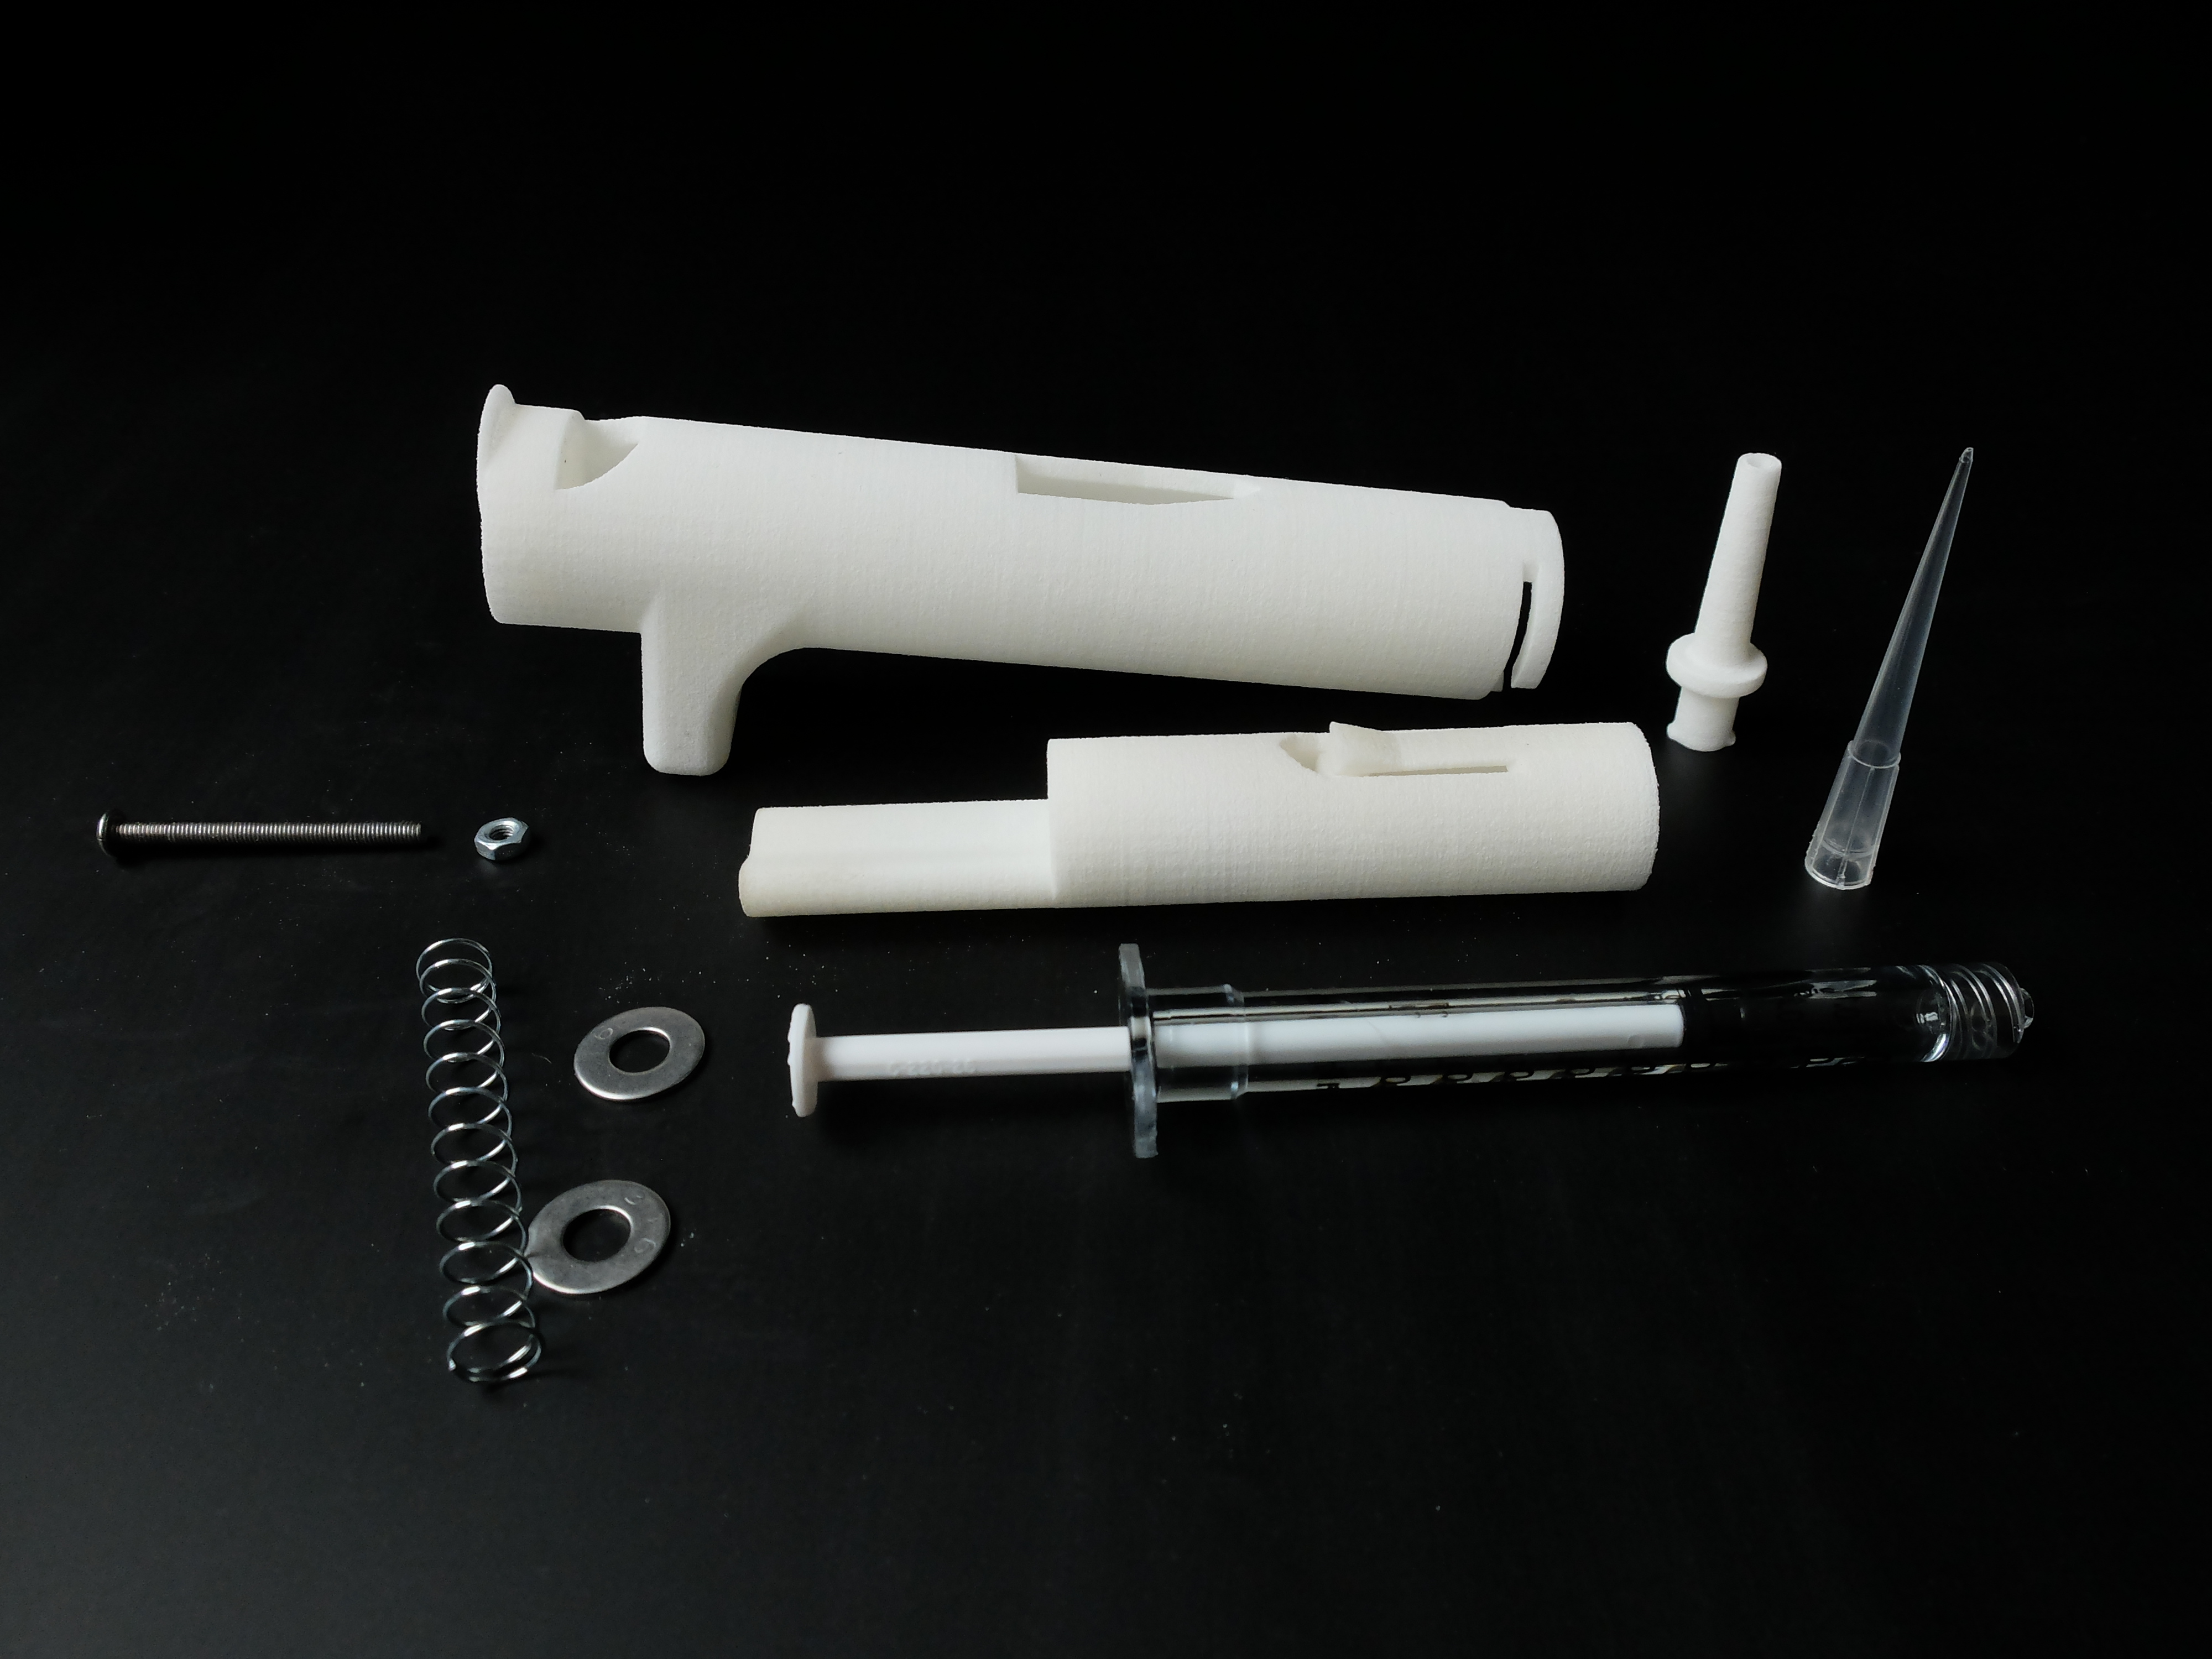
\includegraphics[scale=0.04]{pipette-disassembled.JPG} % take image out for final manuscript
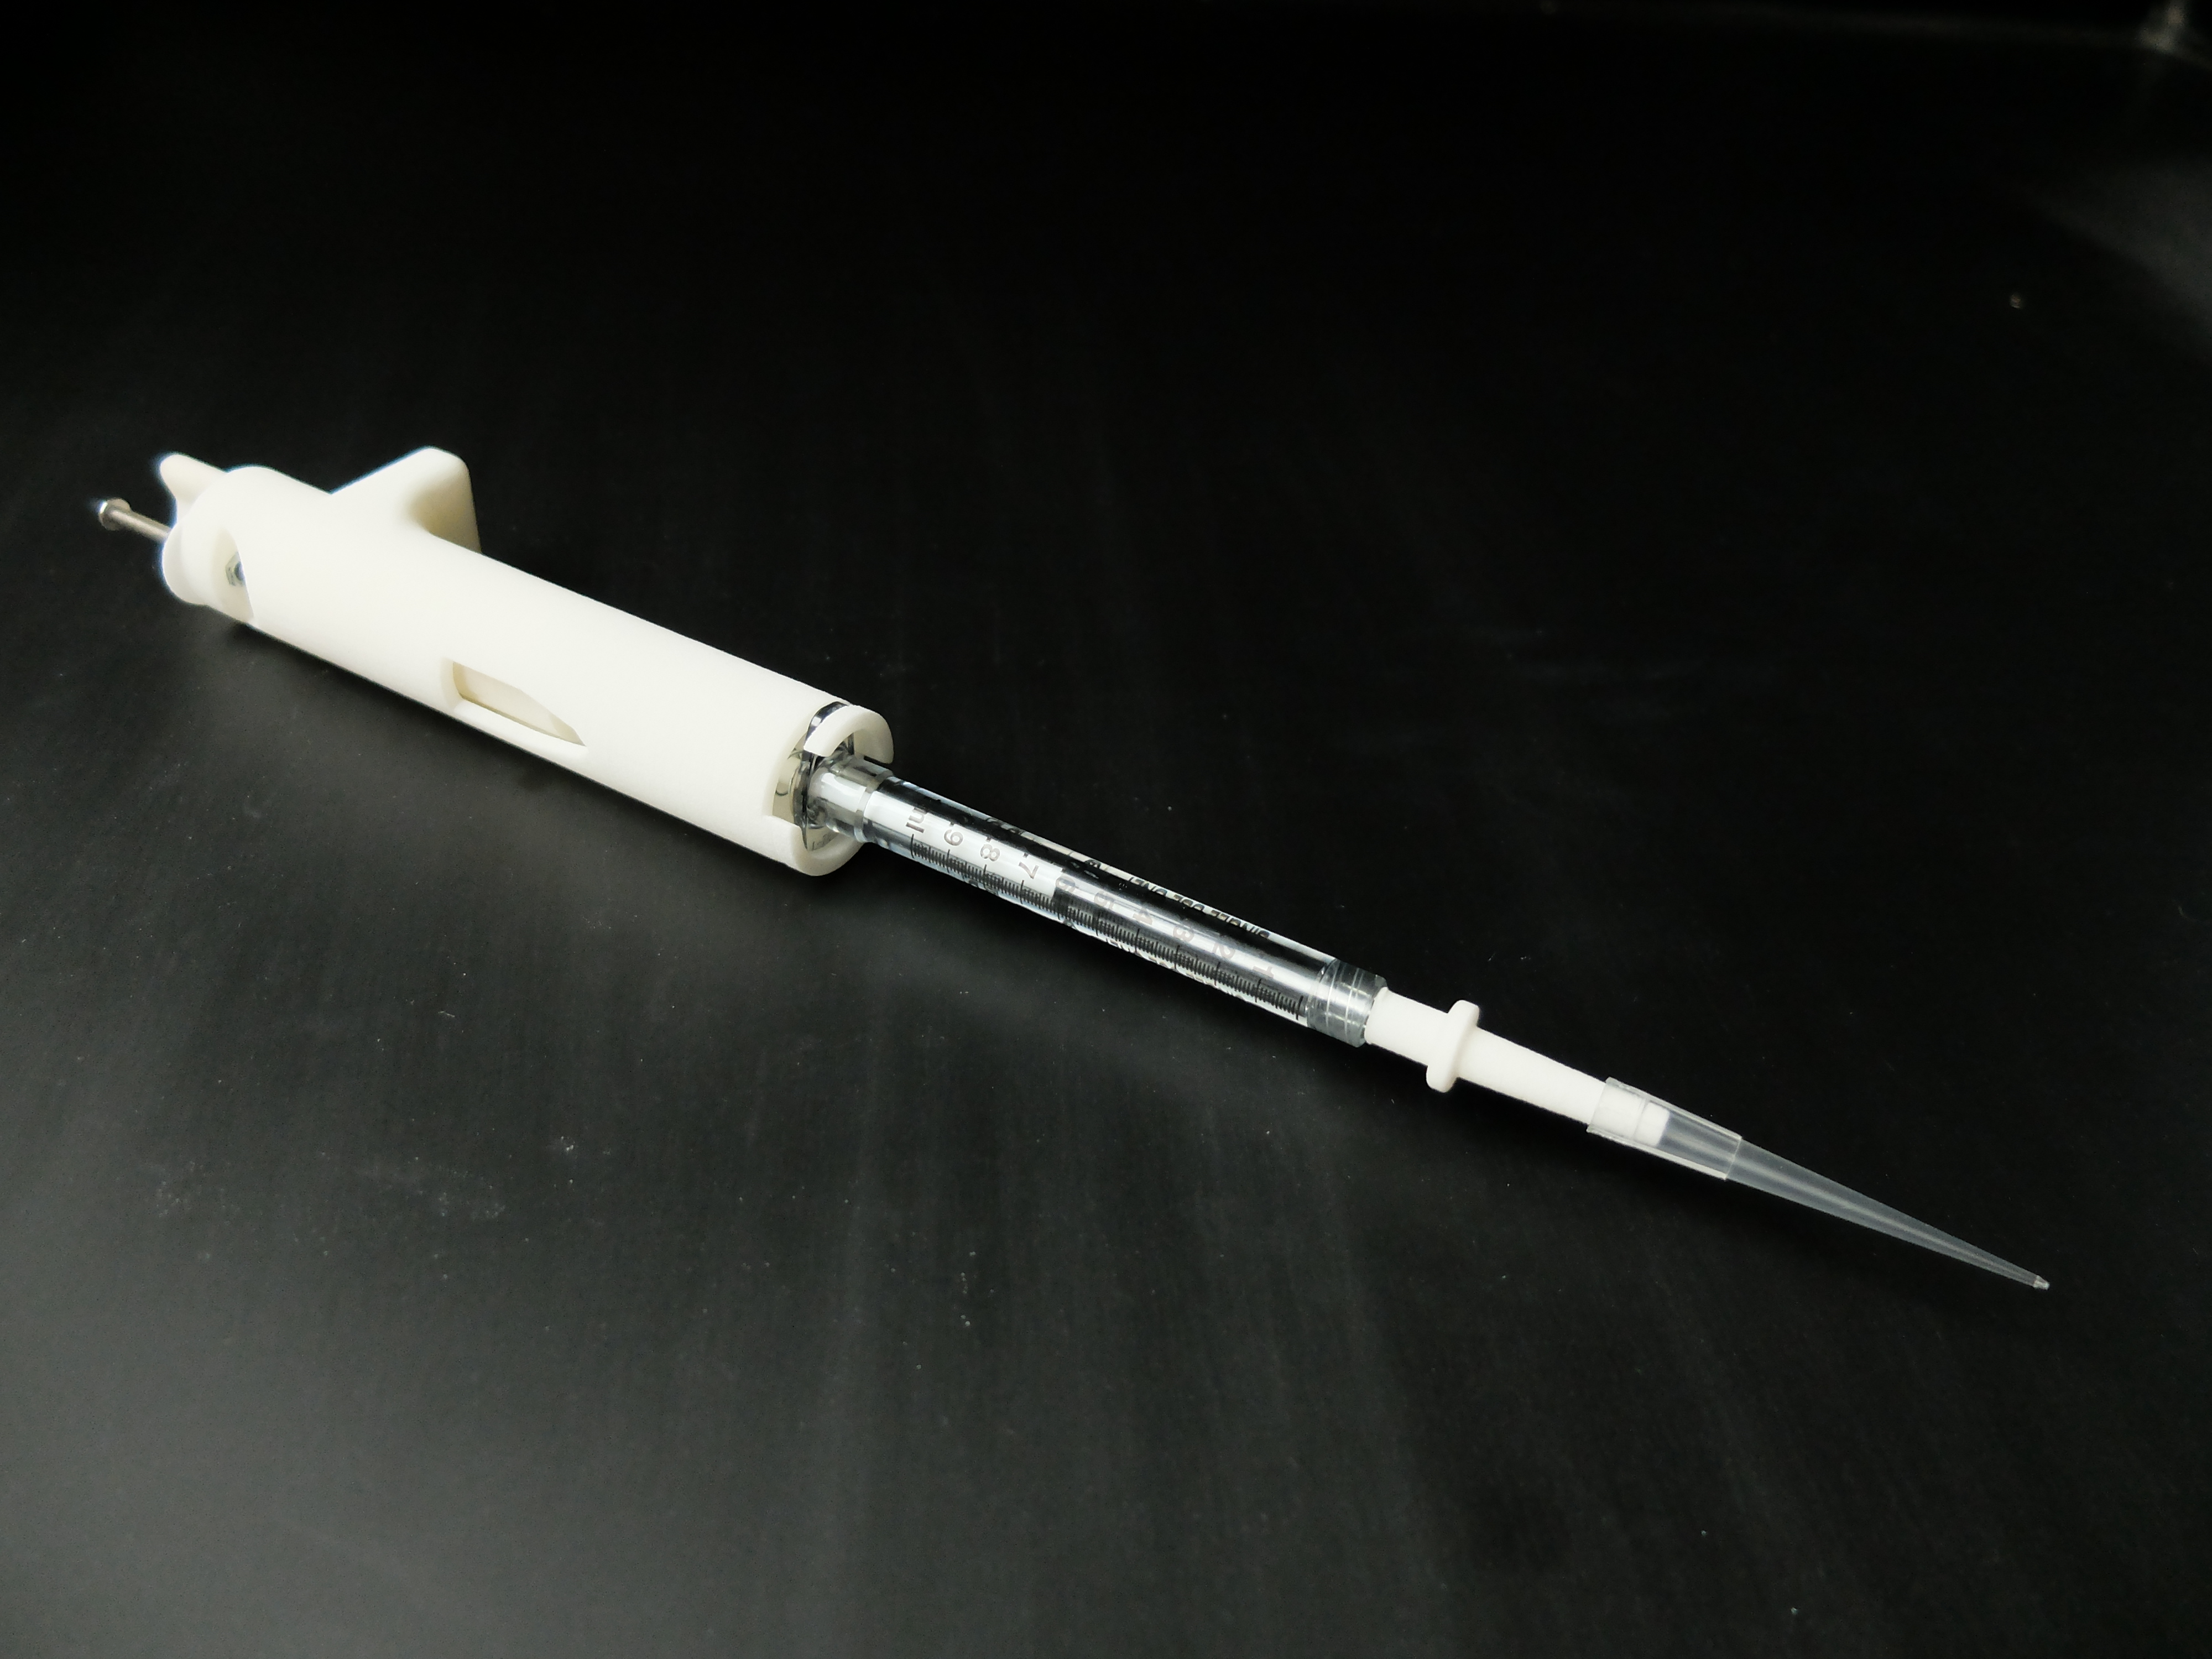
\includegraphics[scale=0.04]{pipette-assembled.JPG} % take image out for final manuscript
\caption{
{\bf Photos of pipette.}  The pipette is composed of three printed parts, a 1 mL syringe and some additional hardware.  
}
\label{photo-parts-figure}
\end{figure}


%\begin{abstract}

%\end{abstract}

%\section{}

\end{document}
